\section{Field Studies}
During the development of the study application, the author tracked himself to select appropriate parameters for the algorithms. The first part of the parameter tuning happened at the Technical University of Munich where the author sat in the large Computer Science building and visited different offices. Once a day the author would eat lunch at the canteen in another building. In Figure \ref{fig:tum-map} the places and the stops at the university are displayed and as can be seen which are very close. Had the radius parameter for finding places been higher, then some of the found places would have been merged into a single place. Here, the place-radius parameter was set to 25 meters, such that individual offices were clustered into one place. Had the distance parameter been higher then some of the offices would have been merged into a single place.\\

\begin{figure}
    \centering
    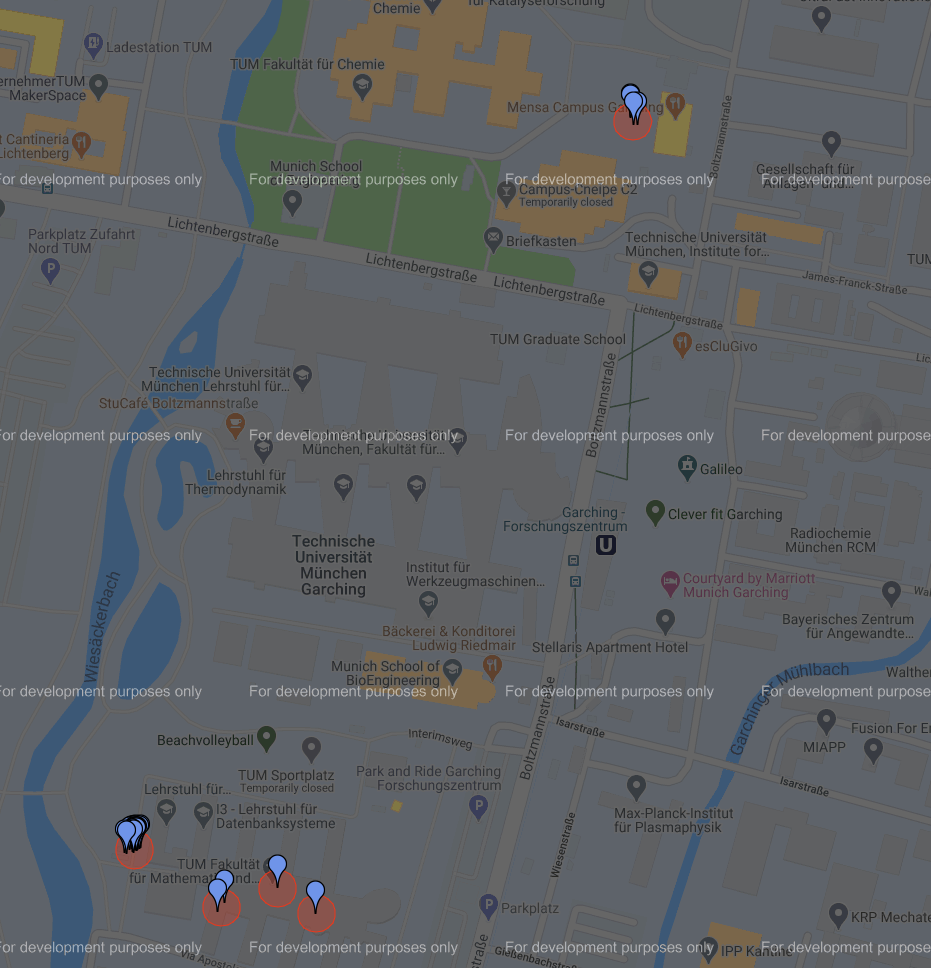
\includegraphics[width=0.7\textwidth]{images/map/map-tum.png}
    \caption{A map of TUM Garching, displaying the Places (red clusters) as well as the Stops which make up these places (blue markers) visited by the author}
    \label{fig:tum-map}
\end{figure}

The author returned to Denmark due to the outbreak of COVID-19, where the parameter tuning continued. Movement patterns varied a lot between the two cities: In Munich the author visited many small places next to each other, whereas in Denmark places were further  apart, and it was found that a place-radius of 50 meters was more suitable.\\

The main study was a small-scale study that ran for 3 weeks between April and May 2020 and included 10 participants (including the author). All the participants were recruited through friends and family and non of them, to the knowledge of the author, were diagnosed with a mental illness. The country of residence was the following:

\begin{itemize}
    \item Denmark (8 participants)
    \item Germany (1 participant)
    \item United Kingdom (1 participant)
\end{itemize}

Since the majority of the participants lived in the Capital Region of Denmark, it was decided to keep the place-radius of 50 meters.\\

The goal of the study was to validate the accuracy of the features produced. In the study the participants used the application discussed in Chapter \ref{chapter:05} to collect their location data and computed mobility features daily. Also, the participants answered a questionnaire daily to get subjective user data. In addition to this, the application also had a diary consisting of 4 questions that the participant had to fill out each day. To make it easy for the user to remember filling out the diary, a reminder was sent to the participants at 8 PM. The time 8 PM was chosen due to being relatively late while still being early enough in the day that people would still be checking their phone. Some people go to bed at 9-10 PM which had to be taken into account.\\


\subsection{Evaluating Features}
The diary questions were related to 3 of the mobility features which were \textit{Number of Clusters}, \textit{Home Stay} and \textit{Routine Index}. The purpose of the questions was to get subjective estimates of the values of these features. Answers were expected to be very subjective since the definition of a place and a routine will vary from person to person. Answers were collected through a diary to evaluate the accuracy of the computed features. The features inquired about had to be easy to formulate as a question such that participants could provide reliable answers. Features such as entropy and location variance were ill-suited for this, whereas Home Stay, Number of Places, and Routine Index were chosen instead. The questions were the following:

\begin{itemize}
    \item[\#1] How many unique places (including home) did you stay at today?
    \item[\#2] How many hours did you spend away from home today? (Rounded-up)
    \item[\#3] Did you spend time at places today that you don't normally visit?
    \item[\#4] On a scale of 0-5, how much did today look like the previous, recent days? (Where 0 means 'Not at all' and 5 means 'Exactly the same')
\end{itemize}

Collecting the subjective \textit{Number of Places} visited, was done by asking the participant how many places they had visited today, including their home. Technically a user may visit no places at all if they are consistently moving throughout the day - but this is highly unlikely.\\

For collecting the subjective \textit{Home Stay} percentage, the participant was asked the inverse question, i.e. how many hours they were \textit{away} from their home today (from which Home Stay can then be calculated later). This question is much easier for the participant to answer, and there was no need to explain to the participant that time spent during the night counts towards the Home Stay. \\

The Routine Index was more difficult to formulate as a question since there is no succinct way of putting it. It was decided upon rating today scale from 0 to 5, where 0 indicates that today looks nothing like previous days and 5 indicating that today looks identical to the previous days. Ideally, the scale should be more fine-grained such as a 0 to 10 scale, however, this would put too much responsibility on the participant to not give arbitrary answers. It may for example be hard to distinguish between a 6 and 7 on a 0-10 scale, whereas distinguishing between 3 and 4 on a 0-5 scale is easier. The information we wished to know was, on a high level, whether or not today looked like the previous days which is still possible with a coarse-grained scale. Question \#3 also related to the Routine Index feature but was not used for later data analysis since it was hard to compare directly to the Routine Index and would require looking at the Hour Matrix instead.

\subsection{Hindrances}
The Coronavirus pandemic leads to countries closing borders and urging people to stay at home as much as possible. This included workplaces shutting down and people had to work from home, as well as places of recreational character such as gyms and restaurants. This had some implications for the study in that people would spend most of their time at home, and they would likely not visit very many places.\\

Also, it was probably not common for most people to go visit new places during the pandemic. However, all in all, the pandemic only shaped the results of the field study and did not prevent the study from taking place at all. Also, the Android platform closed down the access needed for tracking location data in the background without interruption as of February 2020 \footnote{\url{https://nakedsecurity.sophos.com/2020/02/25/android-11-to-clamp-down-on-background-location-access/}}\footnote{\url{https://developer.android.com/training/location/background}}. It was made a priority to conduct the study as soon as possible and therefore the app was released for iOS only, due to time constraints.


